%\newline

%Descripción general del módulo.
%Precondiciones necesarias.
%Por qué existe?
%Qué especificación tiene y cómo se maneja
%Comparación, como manejan los demás trabajos.

\chapter{Diseño del framework}\label{cha:Diseño}

El objetivo principal de este capítulo es describir el diseño del framework propuesto para planificar tareas preemptive en sistemas embebidos heterogéneos. Actualmente existe una gran variedad de planificadores de tareas sobre CPU, la propuesta de esta tesis es presentar el diseño de un framework que ayude a planificar tareas preemptive que se ejecutarán sobre la GPU. El estudio de la planificación de las tareas del CPU queda fuera del contexto de esta tesis.
\newline

Aunque se tomó como base el sistema embebido heterogéneo NVIDIA Jetson TX2, el diseño puede ser aplicado a cualquier dispositivo, siempre y cuando cumpla con la característica descritas en la sección \ref{secc:arqPas}.

\section{Descripción general}

La solución propuesta se basa en las clasificaciones:
\begin{itemize}
    \item \textbf{Por implementación}: \textit{Partición de kernel basada en software}
    \item \textbf{Por planificación}: \textit{Planificación por prioridad.}
    \item \textbf{Por modificación}: \textit{Modificación de código fuente.}
\end{itemize}

En la Figura \ref{fig:diagramabase} se muestra un diagrama de bloques sobre la arquitectura del framework propuesto. Cada uno de los bloques agrupa las bases necesarias para el funcionamiento del framework.
\newline

El framework está dividido en dos zonas de implementación, la primera tiene que ver con aquellas actividades que son propias del Host, como lo es el protocolo de lanzamiento de los kernels (ver sección \ref{secc:lanzamientoKernel}). En el caso del manejo de la memoria, debido a que la tarjeta Jetson TX2 utiliza una arquitectura Pascal (ver sección \ref{secc:arqPas}), se cuenta con una memoria unificada con lo que se simplifican el manejo de las copias de memoria entre el Host y el Device, resultando en que el módulo \textbf{Memoria} (ver sección \ref{secc:memoria}) pertenezca a ambas zonas, también se presenta el almacenamiento de los contextos de cada una de las tareas.

En la zona de implementación del Device encontramos el módulo \textbf{Puntos Preemptive} (ver sección \ref{secc:puntosPreemptive}). Como su nombre lo indica, se plantea la forma en que el framework implementa las suspensiones y reactivaciones de las tareas una vez alcanzado cada uno de los puntos. 
%\newline

Un componente fundamental del framework es el módulo \textbf{Planificador GPU} (ver sección \ref{secc:planificador}), ya que es en donde se proporcionan las pautas para el encolado de las tareas que se ejecutarán en un determinado momento en el Device. Pero para poder realizar dicha prioridad, se plantea el módulo \textbf{Asignación de prioridades}, (ver sección \ref{secc:asigPrioridad}) el cual se encargará de ordenar un conjunto de tareas definiendo sus prioridades dentro de la cola.
%\newline

  \begin{figure}[!]
      %\centering
     % \flushleft
        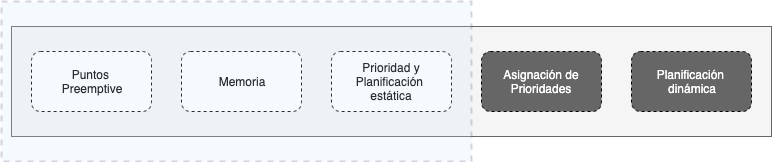
\includegraphics[scale=.6]{diagrama_framework}
        \caption{Esquema del framework para la planificación de tareas preemptive en sistemas embebidos heterogéneos.}
        \label{fig:diagramabase}
    \end{figure}
  %Pero en el momento en el que se requiera tener un método de asignación de prioridades personalizado, es necesario tener un módulo que lo permita. Aunado a esto, si por alguna razón se solicita agregar tareas dinámicamente con el sistema en ejecución, se deben tener mecanismos para manejar cualquier interrupción o actualización de información del planificador. Ambos elementos son necesarios en un framework, pero sus componentes internos se dejarán para ser resueltos como trabajo futuro.
  %Clasificación y tipo de modificación.

Como se detallará más adelante, esta solución no es transparente al programador y es necesaria la modificación del código fuente. 
%Aunque en un inicio pareciera que el rendimiento es inferior al realizar comprobaciones continuas del estado del quantum, la modificación de las bibliotecas del API o el compilador del dispositivo y la implementación de analizadores sintácticos para la lectura de directivas precompiladas salen de las posibilidades de acción del proyecto, por eso no es necesario modificar el código fuente para colocarlas.
%\newline 

El diseño de la asignación de prioridades por el planificador está fuera del alcance de esta tesis (ver sección \ref{secc:asigPrioridad}), pero se puede implementar con la mayoría de la gama de algoritmos del estado del arte (ver sección \ref{sec:AlgoPlan}). Para el estudio de este trabajo se usarán indistintamente los términos kernel y tarea.

  \begin{figure}[!]
      \centering
     % \flushleft
        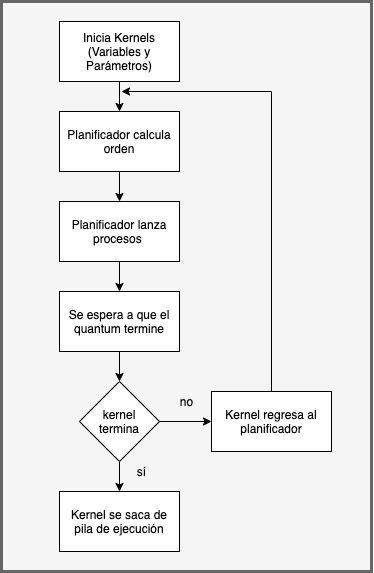
\includegraphics[scale=.74]{flujo}
        \caption{Diagrama del flujo del framework.}
        \label{fig:flujo}
    \end{figure}

\subsection{Precondiciones necesarias} \label{secc:precondiciones}

\begin{itemize}
\item La precondición más importante radica en que el framework debe ser implementado en una aplicación que funciona correctamente, ya que se realizará una modificación en su código fuente para la implementación del modo preemptive.

\item No se permite la memoria dinámica ni compartida entre kernels.

\item No se permiten apuntadores complejos. 

\item No se permite el llamado a funciones no rastreables.

%\item El quantum de las tareas debe ser similar para que aquellas que estén en ejecución terminen en tiempos similares.
\item El quantum deberá ser un parámetro de diseño, es decir establecido para todo el sistema embebido en un archivo de configuración.

\item El número de threads por block debe ser menor o igual a la cantidad de threads disponibles en cada SM.

 \item Los contextos (conjuntos de variables) de cada kernel deben coexistir en la memoria al mismo tiempo para que se puedan ejecutar y suspender en cada punto preempetive.

\item Todas las tareas que soliciten recursos al planificador deben ser preemptive para que en dado caso puedan ser suspendidas, si así lo requiere el balanceo de carga.

\item Para evitar plazos vencidos, el conjunto de tareas de la aplicación debe ser planificable.

\end{itemize}

\section{Puntos preemptive}\label{secc:puntosPreemptive}

%Descripción general del módulo.

La estrategia general en una aplicación acelerada por el cómputo gráfico es implementar más de una función kernel. Pero en el momento en que ejecutamos varias aplicaciones en la GPU habrá alguna que mantenga en sobretiempo los recursos causando así un retraso en la ejecución en general de todo el sistema y sus aplicaciones. Una maniobra de diseño es implementar puntos de control preemptive para tener tiempos de ejecución uniforme independientemente de la duración de cada uno de los diferentes kernels.
\newline

Este módulo permite gestionar la actividad de un kernel a nivel de aplicación, aquí se marca la pauta del punto exacto donde se podrá realizar la administración del contexto de una tarea en ejecución y contará con tres casos principales: si se está iniciando el proceso, si está a la mitad de una ejecución o si ya ha terminado, con esto se podrán liberar los núcleos del GPU para dar oportunidad a otros kernels de consumir recursos.
%\newline

Se propone una serie de puntos de control preemptive que se incluirán explícitamente dentro del código de las aplicaciones que se desean implementar en modo preemptive, definiendo tres estados iterativas del ciclo de vida de un kernel a)inicio, b)en ejecución y c)finalización. 
%\newline

El objetivo de este módulo es resguardar una copia del contexto actual en una estructura de datos llamada Backup cada que se alcance algún punto de control preemptive dentro de un kernel y sea necesario detener su ejecución. De esta manera, cuando se  presente una nueva oportunidad de ejecución sea reanudado justo como si no se hubiera detenido.
\newline

Una vez que una tarea, independientemente del momento de su ciclo de vida en que se encuentre, seguirá ejecutándose en la GPU hasta que complete su cálculo o termine su quantum.
%\newline

Al momento de lanzar la siguiente tarea en la lista de ejecución, y está se encuentre en suspensión preemptive, se inicializan todas las variables necesarias para rearmar el contexto por medio de la copia de datos de la estructura Backup. En caso contrario y se encuentre en el estado inicial del kernel, las variables se inicializarán directamente en código de la aplicación. 
En el algoritmo \ref{lst:inicializa} se presenta la inicialización del kernel mediante la sintaxis CUDA.
\newline
%Qué especificación tiene y cómo se maneja?

Al inicio del algoritmo \ref{lst:declara} la función kernel está ligeramente modificada en sus parámetros, ya que es necesario que reciba la estructura \textit{Backup} en donde se almacena su contexto cuando se presente una suspensión preemptive y también se recibe el apuntador al estado del quantum, dicho valor arrojará \textbf{\textit{true}} cuando se haya concluido el tiempo del quantum.
\newline

Como se mencionó anteriormente, esta solución se basa completamente en software, por lo que se debe estructurar la función kernel para mantener una convención que ayude a mitigar posibles problemas. Todas las declaraciones de variables deberán realizarse en la primera fase, la cual se encuentra en las primeras líneas del kernel.
\newline

Las únicas declaraciones con inicialización permitidas en esta fase son aquellas que designan la posición tanto de los thread como de los blocks dentro de un grid, esto porque  su información es necesaria en cada una de las siguientes fases. La única variable que es necesaria para todos kernels es \textit{id\_block}, que servirá en las siguientes fases para extraer la información de la estructura \textit{Backup}.

\lstinputlisting[style=CStyle, frame=single,label=lst:declara,  basicstyle=\ttfamily\footnotesize, caption=Fase de declaración de variables.]{algorithms/fase_declaracion.c}

Enseguida pasamos a la fase de la inicialización (ver algoritmo \ref{lst:declara}) de cada una de estas variables y como se muestra en el algoritmo \ref{lst:inicializa} nos apoyamos de una estructura \textit{switch-case} con tres casos dependiendo del estado de cada block. Para seleccionar cada uno de los casos debemos leer el valor que se encuentra en la estructura de copia de seguridad, esto porque hay que recordar que el kernel por si solo no sabe si es la primera vez que se ejecuta o está regresando de una suspensión preemptive con un cambio de contexto dentro del sistema.

Los tres estados son:

\begin{itemize}
\item \textit{\textbf{INICIO}}: Se presenta la primera vez que es lanzado un kernel, por lo que el valor inicial debe ser almacenado tanto en la variable local como en su espacio correspondiente en la estructura de copia de seguridad.

\item \textit{\textbf{EJECUCION}}: Se presenta una vez inicializadas las variables en el estado anterior, o cuando el planificador da nuevamente oportunidad de ejecución al kernel en suspensión de ser ejecutado para terminar el procesamiento. Aquí se realiza una transacción de memoria con los datos de la estructura de copia de información a las variables locales para trabajar con la información como si nunca se hubiera suspendido el kernel.

\item \textit{\textbf{TERMINADO}}: Debido a que muchas veces dentro de un kernel hay bloques que finalizan su procesamiento antes que otros, es necesario indicar que esa sección ya terminó y no requiere hacer ningún cálculo.
\end{itemize}

\lstinputlisting[style=CStyle, frame=single,label=lst:inicializa,  basicstyle=\ttfamily\footnotesize, caption=Fase de inicialización.]{algorithms/fase_inicializa.c}

Una vez inicializadas todas las variables podemos realizar el procesamiento objetivo del kernel (ver algoritmo \ref{lst:procesamiento}). Para ello, nuevamente preguntamos a la estructura de copia de seguridad el estado individual de cada block, dependiendo de lo que responda a cada uno, se realiza lo siguiente:

\lstinputlisting[style=CStyle, frame=single,label=lst:procesamiento,  basicstyle=\ttfamily\footnotesize, caption=Fase de procesamiento.]{algorithms/fase_procesamiento.c}

\begin{itemize}
\item \textit{\textbf{INICIO}}: Como se acaba de lanzar el kernel por primera vez, únicamente se cambia el estado del block a \textit{EJECUCION}, y, como ahora se tiene un nuevo valor se puede ingresar al siguiente estado dentro del mismo switch.

\item \textit{\textbf{EJECUCION}}: Al entrar en este caso, en primera instancia se realiza el paso de procesamiento para calcular el kernel original, esto dentro de una estructura \textit{do-while} para que al menos se realice una vez antes de que, o el quantum haya expirado, o se haya completado el procesamiento. Si una de estas condiciones se cumple, el ciclo. Si el kernel se ha completado, el estado del block en el backup se modifica a \textit{TERMINADO} y finaliza ese block sin realizar copia de seguridad para ahorrar tiempo de procesamiento.
En caso de que no haya sido completado, significa que el quantum expiró, por lo que se deben guardar todas las variables locales en su espacio correspondiente designado dentro del backup, dejando el kernel en espera de que el balanceador de carga le indique si continua por otro quantum o entra en suspensión.

\item \textit{\textbf{TERMINADO}}: Cuando se llega a este estado simplemente se termina la ejecución de los hilos de procesamiento.
\end{itemize}

\subsection{Condición de carrera}

La fase de procesamiento (ver algoritmo \ref{lst:procesamiento}) es un procedimiento en el que hay que poner especial atención, ya que es donde se concentra el núcleo de las operaciones del kernel, además es donde se escriben variables compartidas por todo el grid. Por ello, hay que estar conscientes de que se debe evitar la condición de carrera.
\newline

Por esta razón, en el \textit{case INICIO} únicamente el \textit{thread0} de cada block está habilitado para modificar el estado que se guarda en el \textit{backup}. Justo después del cambio de estado se debe esperar en una barrera para que todos los thread conozcan la actualización y no terminen abruptamente su procesamiento.
\newline

Lo anterior se repite en el \textit{case EJECUCION}, cuando se termina el procesamiento, nuevamente sólo el \textit{thread0} está autorizado para editar el contenido del arreglo \textit{estado} en la estructura de copia de información.
\newline

Finalmente, si el procesamiento se realiza con ayuda de contadores, al momento de que expire el quantum, todos los threads deberán suspenderse cuando lleguen al mismo valor, así que, lo más conveniente (en términos de memoria) es guardar sólo una copia de dicho contador. Entonces, una vez más el \textit{thread0} será quien almacene la información en su correspondiente lugar dentro de \textit{thread0} (línea 32).

%%%%%%%%%%%%%%%%%%

  \section{Memoria}\label{secc:memoria}

  \subsection{Almacenamiento del contexto}
%Descripción general del módulo.

Es necesario crear una estructura de datos que guarde las copias de seguridad de los datos pertinentes que en conjunto formen el contexto de un kernel.
\newline

Todos los parámetros y variables que se encuentren dentro de una función kernel deben almacenarse en memoria, por lo que para cada kernel, se debe crear una estructura \textit{ad hoc}.
\newline

\lstinputlisting[style=CStyle, frame=single,label=lst:backup,  basicstyle=\ttfamily\footnotesize, caption=Estructura Backup para almacenar el contexto.]{algorithms/backup.c}

La estructura \textit{backup} (ver algoritmo \ref{lst:backup}) almacena tres tipos de variables, primero todas aquellas variables locales necesarias para resolver el problema original del kernel. Debido a que estas variables son individuales por thread, debe guardarse una copia de cada thread por cada bloque. Esta solución es muy costosa, por lo que se recomienda que la utilización de estas variables sea mínima o nula. En muchos casos, podría almacenarse su contenido directamente en alguna de las variables \textit{resultado} que se pasaron como parámetro.
\newline

El segundo tipo de variables es de tipo contador. Dependiendo del cálculo que se esté realizando, muchas veces se deberán paralelizar \textit{estructuras for} sin dependencia de datos.  Por esta razón, es posible que después de un cierto número de iteraciones se pregunte por el estado del quantum, y ,en ese momento, se realice la suspensión preemptive para todos los threads de un block. Como todos llegaron a ese punto, simplemente, se puede  guardar un valor del contador. En caso de que se estén utilizando contadores que son propiamente controlados por un punto de verificación de quantum, se deberá utilizar el formato de variable local.
\newline

Finalmente, debemos incluir un tipo de variables más que nos ayuden a guardar el estado en que se quedó cada bloque de threads al ser detenido por el planificador.

  \subsection{Variables compartidas}
  
  Al momento de realizar una solución de GPGPU, tenemos que  considerar que existirán variables que deben mantenerse visibles tanto para el host como para el device. En el algoritmo \ref{lst:lanzamiento} de la sección \ref{secc:lanzamientoKernel} tenemos ciertas variables que deben ser compartidas entre ambas unidades de procesamiento. 
    \newline
  
  Aparte de los parámetros que originalmente tienen la función kernel, se agregan dos más: una estructura \textit{backup}, que almacena el contexto cuando se presenta una suspensión preemptive, y ,la bandera \textit{quantum\_expirado}, que nos indica si ya terminó el tiempo máximo de ejecución. Como estamos en el dominio de la memoria unificada, ambos parámetros existirán en la memoria global para que estén disponibles para ambos dispositivos.
  
  
  %%%%%%%%%%%%%%%%%%%%%%%%%%%%%%%%%%%%%%%%%%%%%%%%%%%%%%%%%%%%%

\section{Lanzamiento del kernel}\label{secc:lanzamientoKernel}

El framework plantea dos precondiciones estrechamente relacionadas (ver sección \ref{secc:precondiciones}). La primera, es que el framework planificará un número estático de kernels conocidos desde el inicio y, la segunda, es que el código fuente esté disponible para su adecuación al framework.
\newline

Cada una de las aplicaciones GPGPU que se ejecutarán en el sistema embebido deberán estar agrupadas en cabeceras de C. Al inicio de la ejecución del framework, se ejecutarán las aplicaciones de forma concurrente (Figura \ref{fig:appN_h}) para que todas alcancen el punto en que requieren realizar cálculos en la GPU.
\newline 

  \begin{figure}[!]
      \centering
     % \flushleft
        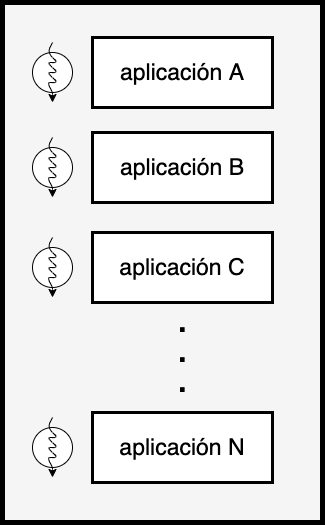
\includegraphics[scale=.3]{appN_h}
        \caption{Aplicaciones en ejecución concurrente en el CPU.}
        \label{fig:appN_h}
    \end{figure}

Se debe encapsular la llamada a la función kernel para que el planificador permita dar el orden de lanzamientos.

Al código de cada una de las aplicaciones se le debe añadir una serie de variables y parámetros extra para que el contexto pueda ser almacenado al alcanzar una suspensión preemptive y planificador eventualmente programe su ejecución. 
%\newline

Entre las variables a incorporar están la definición de la estructura \textit{backup} específica del kernel, también se debe indicar la duración del quantum con \textit{quantum\_time}, una bandera de control para verificar si ya ha expirado el quantum y una bandera que indicará si ya se ha ejecutado completamente el kernel. Finalmente, el planificador dará permiso de que se ejecute el kernel con la variable de control \textit{continuar\_eje}.
\newline

Ahora bien, una vez que se han definido las variables de control, se debe implementar un ciclo que terminará hasta que el kernel sea completado. Dentro debemos inicializar \textit{quantum\_expirado} en \textbf{\textit{false}} para indicar que se tiene tiempo de ejecución. La bandera \textit{continuar\_eje} será modificada por el planificador para permitir la ejecución del kernel. Una vez que sea planificado para su ejecución, se lanzará el kernel  y se esperará el tiempo definido para el quantum. Terminado este tiempo, se cambiará el estado de \textit{quantum\_expirado} a \textit{\textbf{true}} y se sincronizarán todos los threads del kernel con \textit{cudaDeviceSynchronize()} para cerciorarnos de que se terminó la ejecución del grid.

Ahora debemos cambiar el estado de \textit{continuar\_eje} a \textbf{\textit{false}} para que la tarea permanezca suspendida hasta que el planificador permita una nueva ejecución. Finalmente, se pregunta si todos los bloques completaron su trabajo.

\lstinputlisting[style=CStyle, frame=single,label=lst:lanzamiento,  basicstyle=\ttfamily\footnotesize, caption=Algoritmo para lanzamiento del kernel en el lado del host.]{algorithms/lanza_kernel.c}

Para poder determinar si un kernel ha terminado completamente su procesamiento, nos auxiliamos de la función \textit{kc} (Algoritmo \ref{lst:funcionkc}). Simplemente se pasa como parámetro el arreglo \textit{estado} de la estructura \textit{backup} y se pregunta si el estado de todos los blocks es \textit{\textbf{TERMINADO}}, regresando \textbf{\textit{true}}.

\lstinputlisting[style=CStyle, frame=single,label=lst:funcionkc,  basicstyle=\ttfamily\footnotesize, caption=Función kernel completo.]{algorithms/funcion_kc.c}

\section{Planificador GPU} \label{secc:planificador}

El módulo principal del framework es el \textbf{Planificador} (ver figura \ref{fig:Planificador}) porque es donde se realiza toda la calendarización de los kernels a ser ejecutadas en la GPU. Trabaja muy estrechamente con el módulo de asignación de prioridades, el cual da la pauta para poder elegir el orden de los kernels en un momento determinado en el tiempo. 

\lstinputlisting[style=CStyle, frame=single,label=lst:Task,  basicstyle=\ttfamily\footnotesize, caption=Estructura task.]{algorithms/Task.c}

Para poder planificar un conjunto de kernels en la GPU, es necesario conocer las particularidades de la arquitectura del sistema embebido en el que se implementará el framework. Esto es especialmente necesario para que conozcamos el número máximo de threads que pueden estar en ejecución concurrentemente.
\newline

    \begin{figure}[h!]
      \centering
        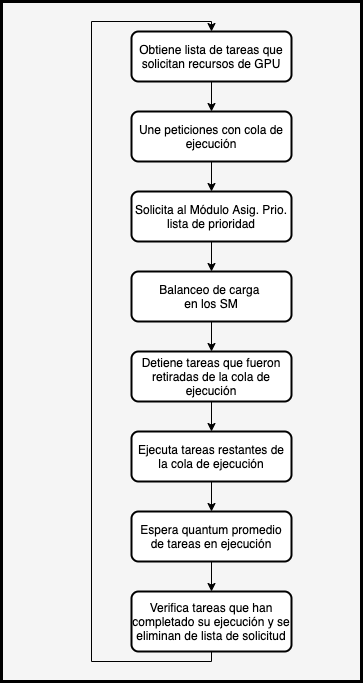
\includegraphics[scale=.6]{Planificador}
        \caption{Diagrama de flujo del planificador.}
        \label{fig:Planificador}
    \end{figure}

Cada uno de los kernels que soliciten recurso de cómputo en la tarjeta gráfica al planificador deberá ser mapeado a una estructura (algoritmo \ref{lst:Task}), la cual tendrá almacenados los parámetros necesarios para su ejecución, así como información relevante para la asignación de su prioridad en un instante de tiempo.
\newline

El algoritmo \ref{lst:planificador} muestra la manera en que deberá guiarse el programador para implementar el planificador, primero se obtiene la lista de tareas \textit{sol} que solicitan los recursos del GPU y las une con aquellas que ya se tenían en la cola de ejecución \textit{R}, esta cola contiene tanto las tareas que en una ejecución fueron beneficiadas de consumir recursos como aquellas que se mantienen en estado de espera.
\newline

Se llama al módulo Asignación de Prioridad (ver sección \ref{secc:asigPrioridad}) para que devuelva la cola ordenada por prioridad \textit{r} (el orden depende del algoritmo de asignación de prioridades en tiempo real seleccionado).
\newline

\lstinputlisting[style=CStyle, frame=single,label=lst:planificador,  basicstyle=\ttfamily\footnotesize, caption=Función planificador.]{algorithms/planificador.c}

La cola \textit{r} se envía a un balanceador de carga que ayudará a la maximización de la planificación de tareas ejecutables en un quantum. Posteriormente, detendrá la ejecución de aquellas que deban resguardar su contexto en la iteración actual \textit{j} para darle lugar a un kernel con mayor prioridad.
Se esperará un determinado número de quantums (el estudio del quantum más apropiado queda fuera del contexto de esta tesis) y una vez alcanzado el plazo límite, se eliminarán de la cola \textit{R} aquellas tareas que completaron su ejecución en la iteración \textit{j}. 


    \begin{figure}[!]
      \centering
        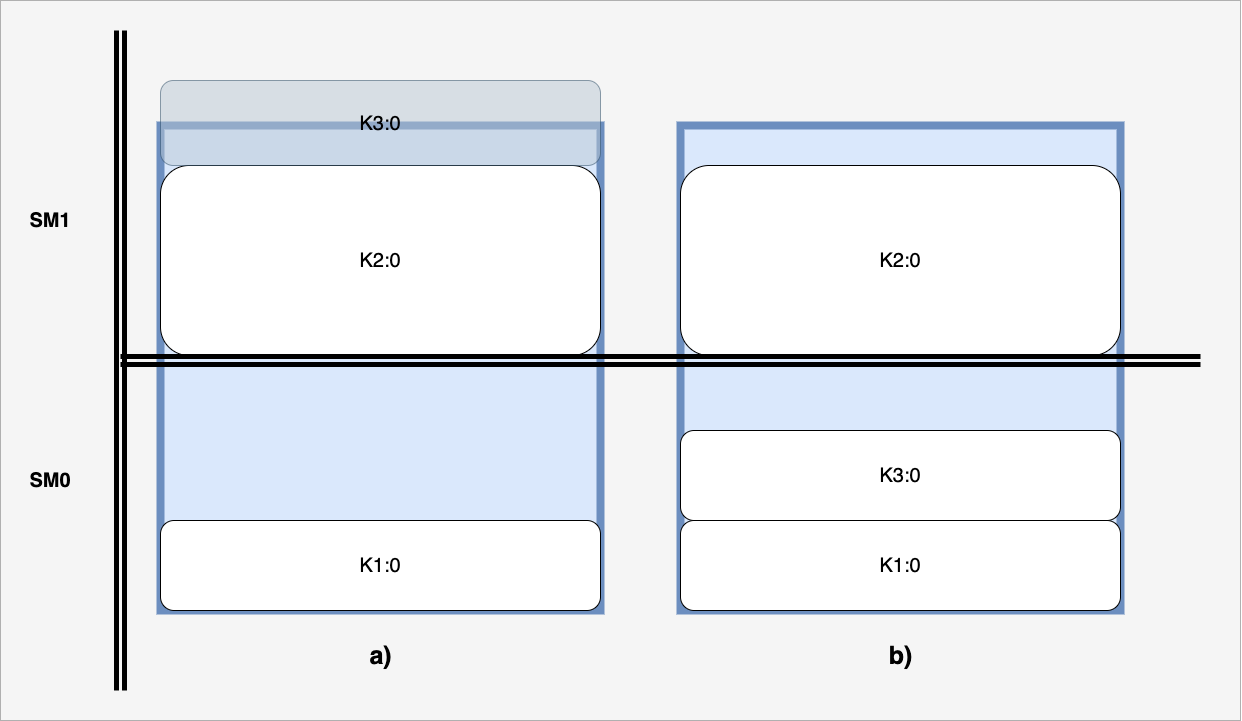
\includegraphics[scale=.30]{Balanceo}
        \caption{Diagrama de balanceo de carga de kernels en los SM.}
        \label{fig:Balanceo}
    \end{figure}
    
\subsection{Balanceador de carga} \label{secc:balanceador}

Bajo suposición de la asignación de carga de trabajo, todas las tareas son preemptive debido a que por decisiones inherentes del hardware muchas veces no podrán asignarse aunque haya espacio para su ejecución.
\newline

Como se mencionó en el capítulo \ref{cha:TrabajoRelacionado} el orden de lanzamiento de los kernel a la GPU afecta la forma en que serán asignados a los SM. Por ejemplo, en el escenario \textbf{a)} (ver figura \ref{fig:Balanceo}). Primero se lanza \textbf{K1}, seguido de \textbf{K2} y al final \textbf{K3}, dando como resultado el desperdicio de recursos y que no sea posible ejecutar el kernel \textbf{K3}. Sin embargo, si se modifica el orden de asignación a los SM, se puede optimizar el reparto de tareas en las localidades, como lo vemos en el ejemplo \textbf{b)}.
%\newline

Por esta razón, se ideó un balanceador de carga (ver algoritmo \ref{lst:Balanceador}) que permitirá la maximización de la planificación de tareas ejecutables en un quantum rellenando los SM hasta que se asigne la mayor cantidad de tareas posibles para su operación en concurrente.
\newline

Como se ha visto a lo largo de este trabajo, la asignación de recursos para la ejecución de kernels en la tarjeta gráfica no es algo trivial, por lo que fue necesario diseñar un balanceador de carga (ver figura \ref{fig:Balanceador1}) que tomara en cuenta las características propias del sistema utilizado como caso de estudio.
\newline

La lógica de asignación de tareas a los SM se basa en colocar la mayor cantidad posible de kernels en concurrente pero sin realizar muchos cambios de contexto.
\newline

    \begin{figure}[!]
      \centering
        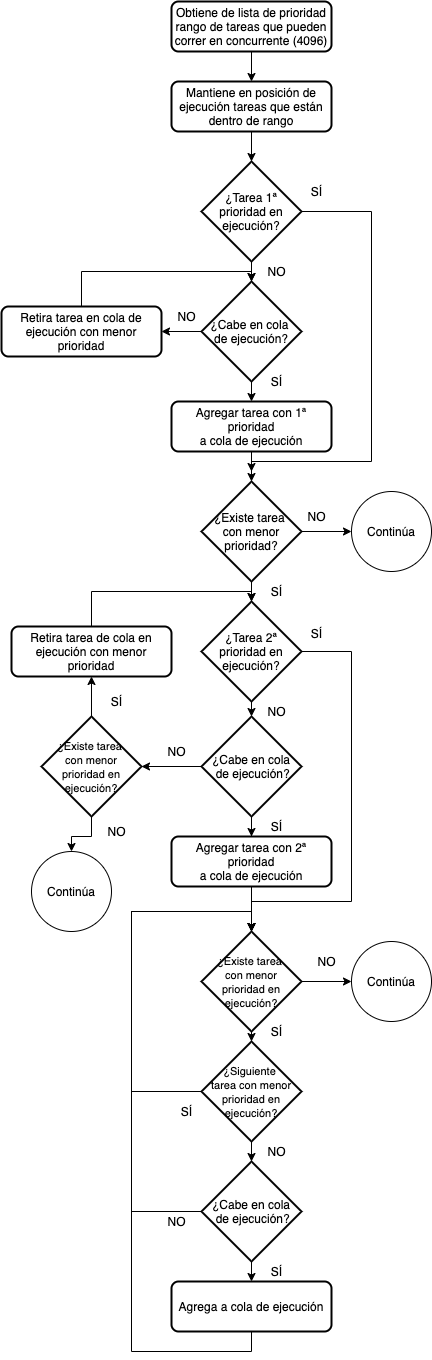
\includegraphics[scale=.75]{Balanceador}
        \caption{Diagrama de flujo del balanceador de carga.}
        \label{fig:Balanceador1}
    \end{figure}

\lstinputlisting[style=CStyle, frame=single,label=lst:Balanceador,  basicstyle=\ttfamily\footnotesize, caption=Balanceador de carga.]{algorithms/balanceoCargav4.c}

El balanceador obtendrá de la lista de prioridad \textbf{r} el rango de tareas que en caso hipotético pueden ser ejecutadas en los SM en concurrente.
La lista de prioridad ahora estará dividida en 3 secciones. La primera estará compuesta por las \textbf{n} tareas que encabezan la lista, donde \textbf{n} es un parámetro de diseño que dependiendo de las características deseadas propias del sistema a implementar. 
La segunda sección contiene las tareas de mediana prioridad, aquellas que no se encuentran dentro de las primeras \textbf{n}, pero que se encuentran dentro del rango de posible ejecución. 
Finalmente, las tareas de baja prioridad, aquellas que quedaron fuera del rango.
\newline

El balanceador primero verificará si existen warps disponibles para la ejecución de las tareas de la lista de prioridad. Siempre lo hará en orden, de mayor a menor prioridad. Si alguna tarea ya se encuentra en ejecución, se tratará de dejarla en su posición dentro de los SM para evitar, en la medida de lo posible, los cambios de contexto que son los eventos que mayor tiempo requieren para su ejecución.
\newline

\lstinputlisting[style=CStyle, frame=single,label=lst:BalanceadorBloques,  basicstyle=\ttfamily\footnotesize, caption=Bloques del balanceador.]{algorithms/balanceoBloques.c}

Si la tarea no se encuentra actualmente en ejecución y está catalogada como de alta prioridad, se le buscará espacio dentro de las tareas de baja prioridad primero. En primera instancia (ver algoritmo \ref{lst:BalanceadorBloques}), se pregunta si existe una tarea de baja prioridad con la misma cantidad de warps, si es así, se intercambia el contexto de las tareas para que la que tiene mayor prioridad se ejecute en su lugar. 
En caso que no encuentre un par, se buscará alguna otra que ocupe un número mayor de warps (siempre prefiriendo aquella más cercana en número de warps). Si no se encuentra, ahora se pregunta si existen tareas de baja prioridad vecinas que sumadas tengan mayor o igual cantidad de warps. 

En caso que la tarea no hubiera podido entrar en los warps ocupados por las de baja prioridad, se comienza a preguntar con las de prioridad media. Si existe un tarea de mediana prioridad con misma cantidad warps, realiza el cambio de contexto, si no, busca aquellas tareas con una cantidad mayor de warps, recordando siempre que se preferirá la tarea más cercana en warps pero que sea de menor prioridad, ya que una de menor prioridad no puede solicitar los recursos de una tarea de mayor prioridad. 
El último paso es preguntar por la existencia de una tarea de media prioridad que como vecina a una tarea de baja prioridad, y que sumadas posean una cantidad mayor o igual de warps.
\newline

Para el caso de la asignación de tareas de mediana prioridad, se realizará únicamente las evaluaciones con las de baja prioridad. Y, con el fin de maximizar la utilización de los recursos de GPU, los warps disponibles se repartirán entre las tareas de menor prioridad, siempre en orden de prioridad.
\newline

A continuación se muestran algunos de los diversos escenarios en forma de casos de estudio que pueden aparecer durante la planificación. Cada caso ilustra el balanceo de cargas a ejecutar en un quantum. 
\newline

 \begin{table}[h!]
      \begin{center}
            \footnotesize
        \begin{tabular}{|m{2cm}|m{9cm}|}
         \hline
         \cellcolor{lightgray}\textbf{Caso I} & El planificador permite que las tareas continuen con su ejecución otro quantum sin ser interrumpidas.\\ 
         \hline
          \cellcolor{lightgray}\textbf{Caso II} & Se modifica la lista de prioridad y kernels de baja prioridad ahora son de mediana prioridad.\\ 
         \hline  
         \cellcolor{lightgray}\textbf{Caso III} & Kernels han completado su ejecución y deben ser sacados de la lista de prioridad.\\ 
         \hline
         \cellcolor{lightgray}\textbf{Caso IV} & Kernels de alta prioridad tienen preferencia sobre los de mediana prioridad.\\ 
         \hline
         \cellcolor{lightgray}\textbf{Caso V} & Kernels de alta prioridad que no estaban originalmente en ejecución realizan una gran cantidad de movimientos para asegurar su ejecución.\\ 
         \hline
           \end{tabular}
        \caption{Descripción de casos del balanceador de carga.}
        \label{tab:Casos}
      \end{center}
    \end{table}

    \begin{figure}[h!]
      \centering
        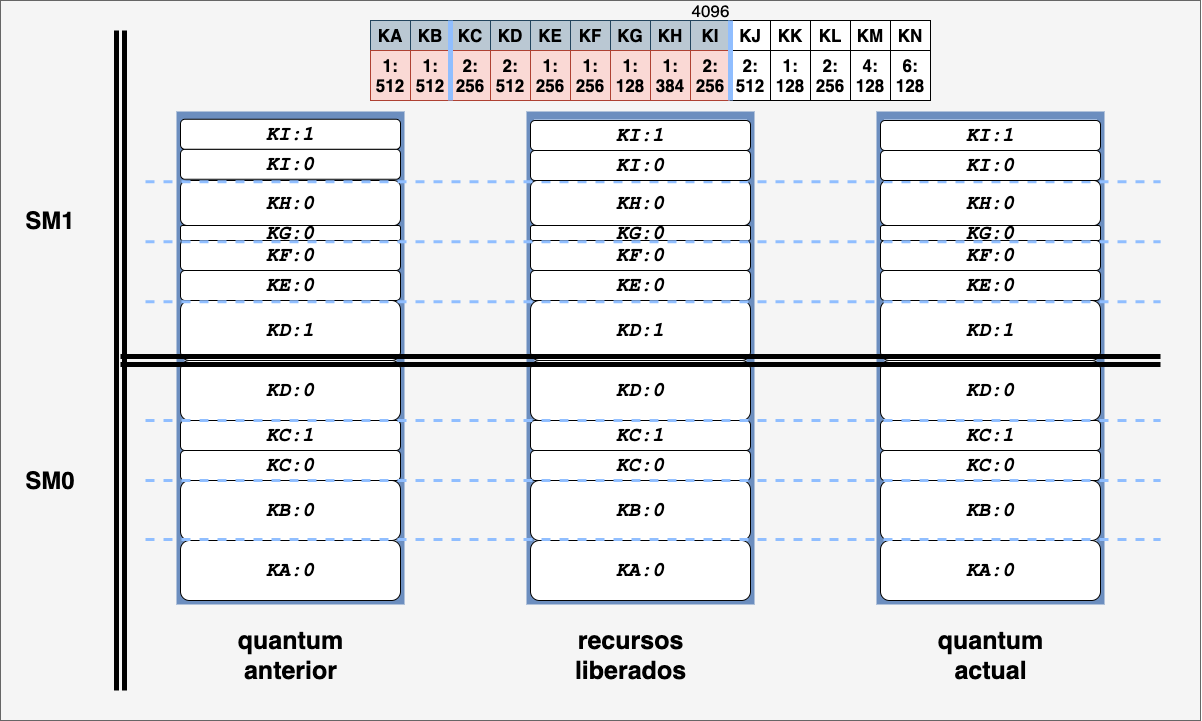
\includegraphics[scale=.35]{C1Balanceo}
        \caption{Caso I Kernels mantienen su prioridad en la siguiente iteración.}
        \label{fig:C1Balanceo}
    \end{figure}

La tabla \ref{tab:Casos} muestra una descripción de lo que cada caso pretende ilustrar. Para los ejemplos se tiene \textbf{n = 2} tareas de alta prioridad.
\newline
   
El diagrama cuenta con la lista de prioridad ordenada y dividida en las tres secciones de prioridad, y al final de la segunda la cuenta de threads que entraron en el rango de posible ejecución.

Se utiliza un código de color para facilitar la visualización de los eventos ocurridos, se sombrean de gris aquellas tareas que originalmente estaban en ejecución y resultaron nuevamente como posible ejecución, en color verde aquellas que entraron como posible ejecución pero no lo estaban en el quantum anterior, y como amarillo aquellas que salieron del rango de posible ejecución para el nuevo quantum. 
También se sombrearon de rojo aquellas tareas que después del balanceo de carga lograrán ejecutarse en el quantum actual.
\newline

El \textbf{Caso I} (ver figura \ref{fig:C1Balanceo}), representa un escenario en donde la totalidad de las tareas que estaban ejecutándose en el quantum anterior no terminaron terminaron su ejecución, pero vuelven a quedar en la posición de mayor prioridad en la lista. Puesto que ninguna tarea tuvo que ser sacada de ejecución, se les dará oportunidad de un siguiente quantum sin necesidad de detenerse, guardar su contexto y relanzarse.
\newline

    \begin{figure}[h!]
      \centering
        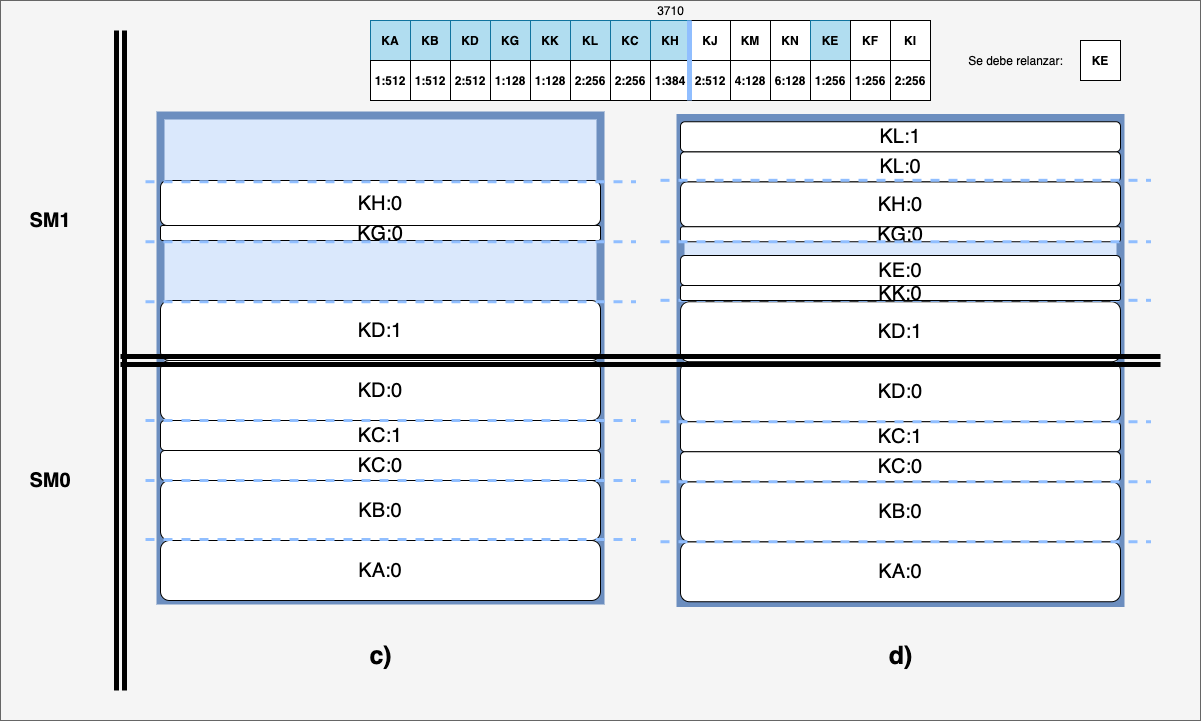
\includegraphics[scale=.35]{C2Balanceo}
        \caption{Caso II Kernels suben de prioridad.}
        \label{fig:C2Balanceo}
    \end{figure}
    
Una vez terminado el quantum de la iteración y recalculando la lista de prioridades, observamos que se presenta el \textbf{Caso II} (ver figura \ref{fig:C2Balanceo}), donde algunas de las tareas ahora cambiaron el orden en la lista de prioridad. 
Ahora entraron a la sección de posible ejecución las tareas \textbf{KK} y \textbf{KL}, mientras que salieron las tareas \textbf{KE}, \textbf{KF} y \textbf{KI}. El kernel \textbf{KK} comienza a buscar un lugar dentro de loa SM para ser ejecutada, y la tarea de baja prioridad que más se ajusta a sus características es \textbf{KF}, por lo que se mapean sus recursos en su nueva posición. 
La siguiente tarea en busca de recursos ahora es \textbf{KL}, y justo empata con la posición de \textbf{KI}, intercambiando así el mapeo de sus recursos. Finalmente, \textbf{KE} como no tuvo que ser movida de su posición tiene oportunidad de ejecutarse nuevamente en este quantum a pesar de ser de baja prioridad.
\newline

    \begin{figure}[h!]
      \centering
        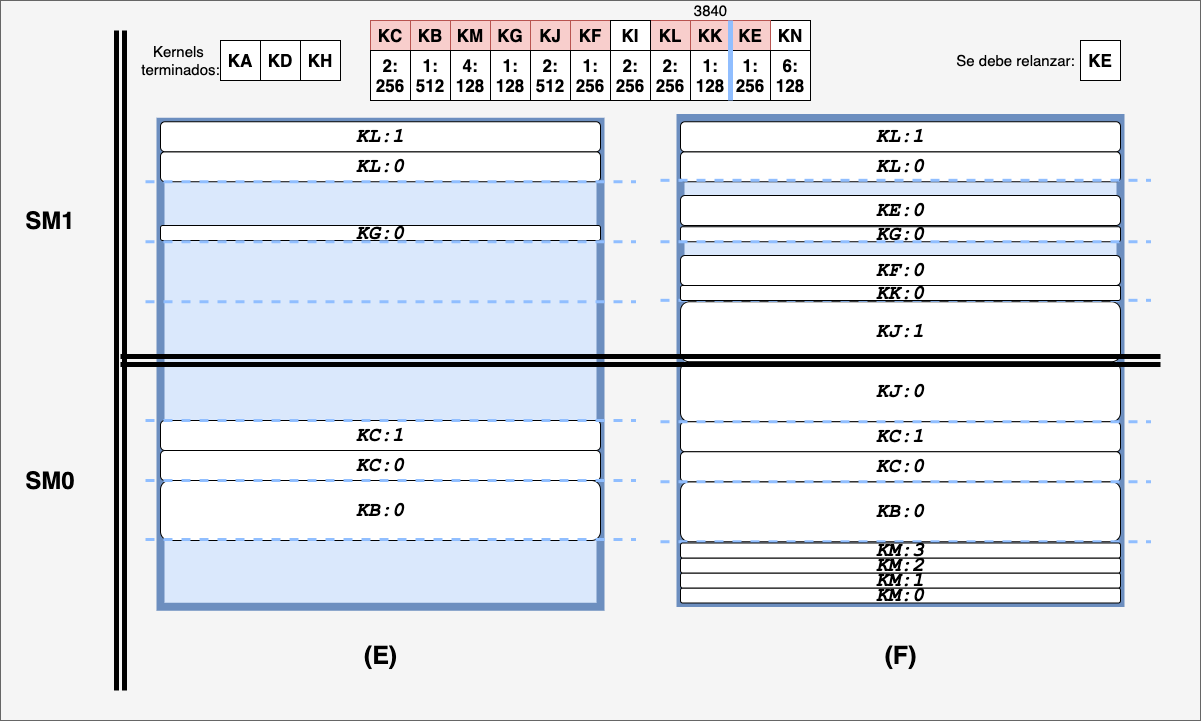
\includegraphics[scale=.35]{C3Balanceo}
        \caption{Caso III Kernels que completaron su ejecución.}
        \label{fig:C3Balanceo}
    \end{figure}

Continuando con el ciclo de vida del planificador, se presenta un posible \textbf{Caso III} (ver figura \ref{fig:C3Balanceo}) donde las tareas \textbf{KA}, \textbf{KD} y \textbf{KH} han completado su ejecución, por lo que son eliminadas de la lista de ejecución. Con esto, la cola de ejecución ha sido modificada tanto en orden como en longitud. Las tareas \textbf{KM}, \textbf{KJ}, \textbf{KF} y \textbf{KI} ahora figuran dentro del rango de las posibles ejecuciones. 
La tarea \textbf{KM} se ajusta perfectamente en los recursos liberados por \textbf{KA} por lo que es mapeada sin problemas. Ocurre lo mismo con \textbf{KJ} ya que quedan libres los warps que ocupaba \textbf{KD} y también \textbf{KF} ocupa los que originalmente pertenecían a \textbf{KH}.
Pero no así con \textbf{KI}, ya que después de preguntar, no se encuentra una ranura para su ejecución, con lo que en este quantum se queda en la lista de espera.
\newline

\begin{figure}[h!]
  \centering
    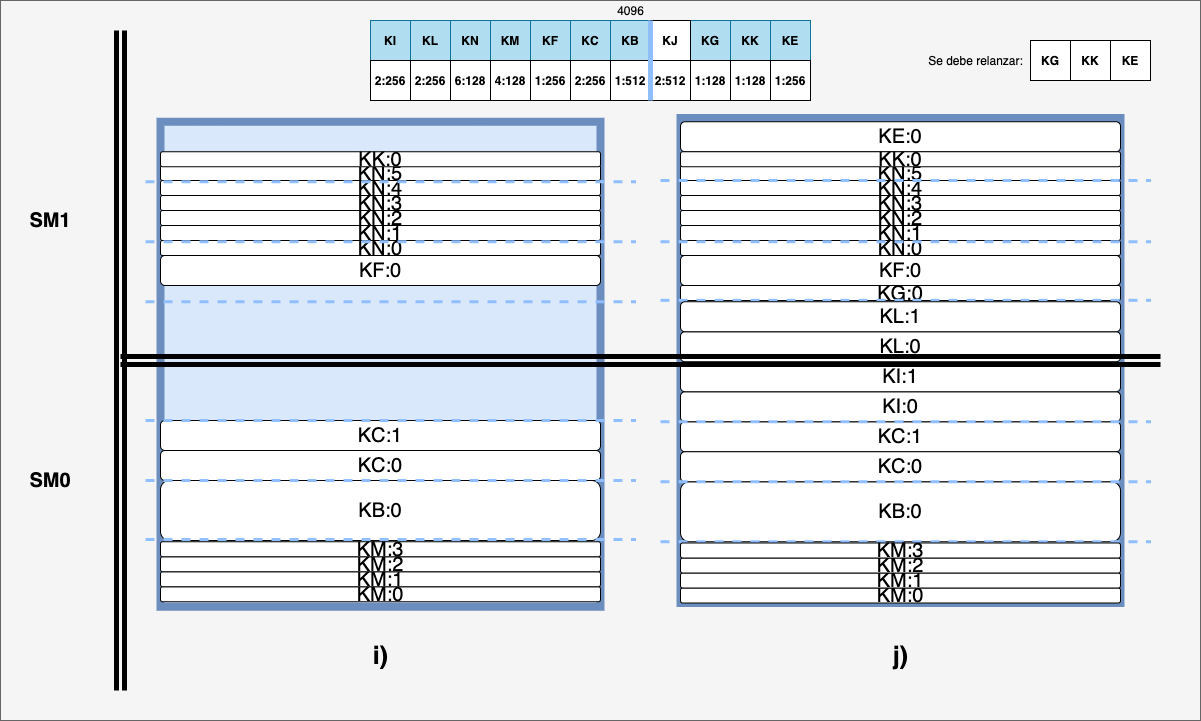
\includegraphics[scale=.35]{C4Balanceo}
    \caption{Caso IV Kernels de alta prioridad tienen preferencia.}
    \label{fig:C4Balanceo}
\end{figure}

En el caso \textbf{Caso IV} (ver figura \ref{fig:C4Balanceo}) la tarea \textbf{KN} ahora se encuentra dentro de las tareas de las tareas de alta prioridad, \textbf{KI} dentro de las de mediana prioridad y las tareas \textbf{KG}, \textbf{KL} y \textbf{KK} ahora son de baja prioridad. Debido a que \textbf{KN} es de alta prioridad, intercambio sus recursos con \textbf{KJ} ya que no hubo otra opción para su mapeo. 

Todas las demás tareas mantuvieron su posición, incluso siendo de baja prioridad, pero imposibilitando a \textbf{KI} ejecutarse.
\newline

\begin{figure}[h!]
      \centering
        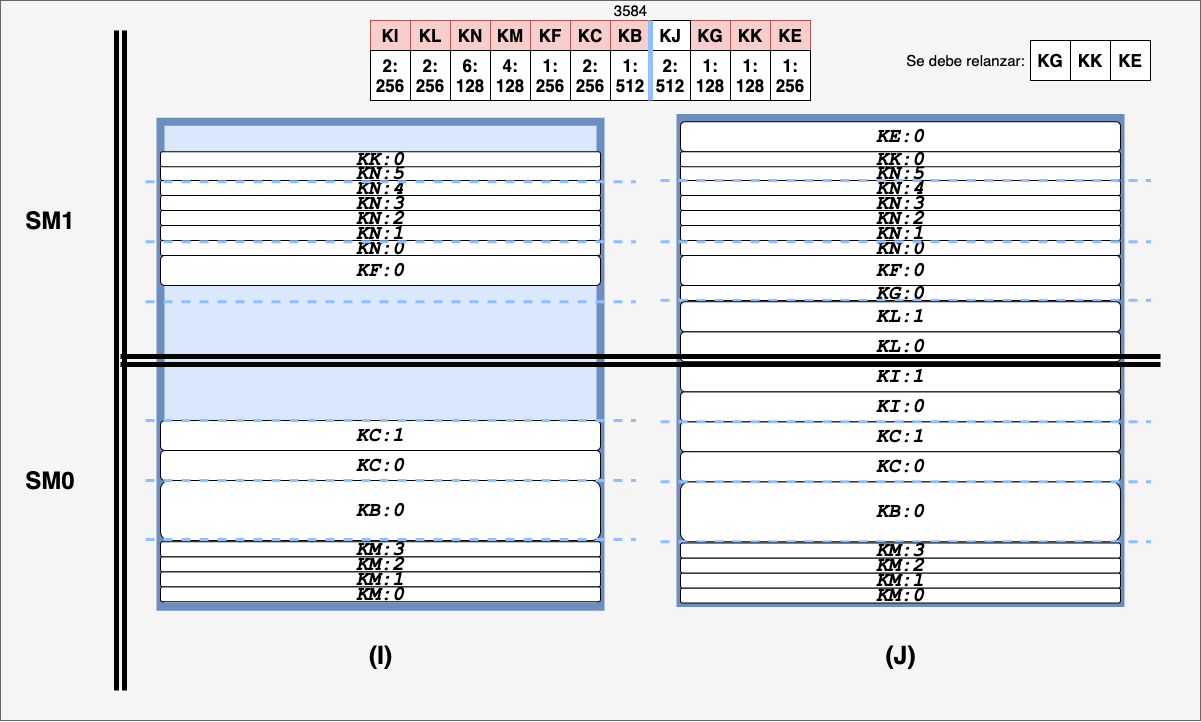
\includegraphics[scale=.35]{C5Balanceo}
        \caption{Caso V Kernels de alta prioridad que no estaban en ejecución.}
        \label{fig:C5Balanceo}
    \end{figure}

En \textbf{Caso V} podemos observar en la figura \ref{fig:C5Balanceo} que en el quantum anterior existen kernels muy dispersos por los SM, pero al momento de obtener la lista de prioridad las tareas \textbf{KT} y \textbf{KU} encabezan la cola, ambas siendo de alta prioridad. 
Al momento de seguir con la metodología de balanceo de carga, se intercambian las tareas \textbf{KW}, \textbf{KS}, \textbf{KY} y \textbf{KR} por las de mayor prioridad, y como fueron desplazadas a una nueva posición, deben ser relanzadas para que tomen los nuevo recursos que se les asignaron.  
\newline

Finalmente, se presentará en la siguiente sección el procedimiento para asignar la prioridad a las tareas y generar la lista de prioridad que recibe el Módulo Planificador GPU

%----------------------------------------    
\section{Asignación de prioridades} \label{secc:asigPrioridad}

Al tener como módulos separados tanto el planificador como la asignación de prioridades, nos da la flexibilidad de poder implementar diferentes algoritmos de tiempo real (ver sección \ref{sec:AlgoPlan}).
\newline

Para el diseño de este framework, se tomó como base el uso de algoritmos de asignación de prioridades en tiempo real de soporte monoprocesador, aunque no se descarta la posible implementación de aquellos que trabajan con multiprocesadores y subconjuntos de tareas. En este caso se asegura la ejecución de al menos dos tareas en concurrente en la tarjeta gráfica.
\newline

Dependiendo de las particularidades de cada algoritmo, se requerirá diferente información sobre la tarea a planificar, dichos parámetros podrán modificarse en la estructura (algoritmo \ref{lst:Task}) que mapea a las tareas.
\newline

Este módulo generará una lista de prioridad ordenando las tareas de mayor a menor, según sea el caso.
\newline

A cada iteración del planificador se asigna una prioridad a las tareas que actualmente están solicitando recursos de la GPU dependiendo de variables temporales. La planificación de las tareas del CPU pudieran ser manejadas por el sistema operativo o algún otro componente, pero su estudio está fuera del contexto de esta tesis.
\newline

El ejemplo de un posible algoritmo para la asignación de la prioridad de las tareas se muestra en el capítulo \ref{cha:Rendimiento}.